\section{Project Results}
\label{sec:project_results}
In the following chapter, the author analyses the results obtained from the hardware and software developed in this thesis project. The candidate successfully executes the minimal Linux OS in real hardware using the developed System on a chip. All the results obtained in this thesis which communicate with the FPGA board or the SoC testbench, are executing the developed \textit{Console} program. The hardware components comprising the SoC differ depending on the software needs.

The objective of this thesis project was to run an Operating System in the \textit{IOb-SoC-Linux}. Table \ref{tab:time_os} presents how much time it takes to build the complete OS with the command "make build-OS". The "real" time is the time that passes since the user executes the command until it finishes. The "user" time is the time the CPU takes while executing operations in the user space. The "user" time is bigger than the "real" time because it counts the time passed in each CPU core. Part of the compilation of the RootFS and the kernel is done in parallel using two cores.

\begin{table}[!ht]
    \centering
    \begin{tabular}{ll}
    real & 4m29,570s \\
    user & 8m12,039s \\
    sys  & 0m56,887s
    \end{tabular}
    \caption{Time it takes to build the OS.}
    \label{tab:time_os}
\end{table}

The OS size is to big to run in the FPGA internal memory. The \textit{OpenSBI} bootloader is 90896 Bytes. The device tree blob is 1669 Bytes. The Linux kernel is 4426152 Bytes. Lastly the root file system is 1142733 Bytes. The memory has to have at least 8 MB ($2^23$) to store all this software. However, the Linux kernel needs a bigger memory where it can store virtual memory pages and execute the different application processes. The device tree source describes the system had 512 MB of available memory. Consequently, the author had to implement the \textit{IOb-SoC-Linux} on the FPGA with access to the external memory. The internal memory could never be as big as 512 MB.

In figures \ref{fig:start_bootloader_sim} and \ref{fig:end_bootloader_sim} the reader can see the start of the OS simulation with \textit{Verilator}.

\begin{figure}[!ht]
    \centering
    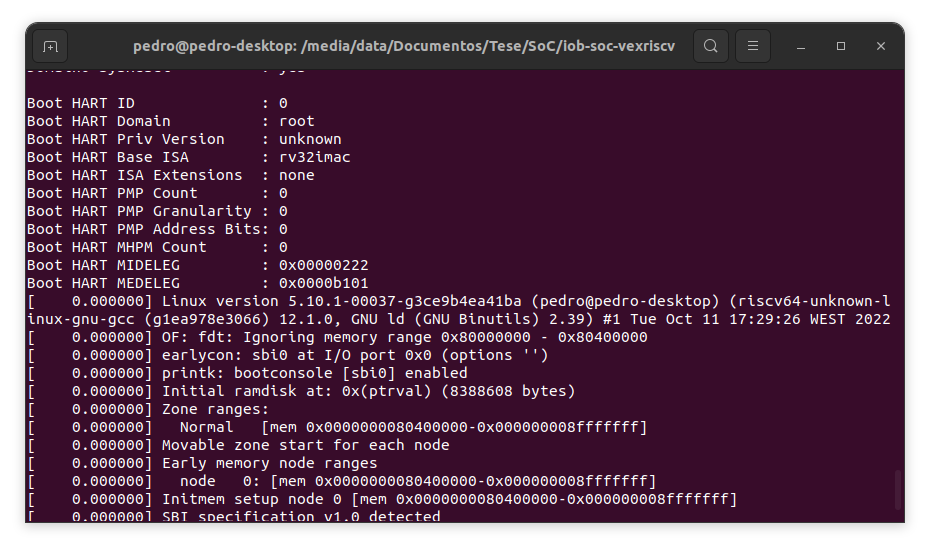
\includegraphics[width=0.5\textwidth]{../images/start_Linux_sim.png}
    \caption{\textit{iob-UART16550} and \textit{iob-PLIC} properties.}
    \label{fig:start_bootloader_sim}
\end{figure}
\begin{figure}[!ht]
    \centering
    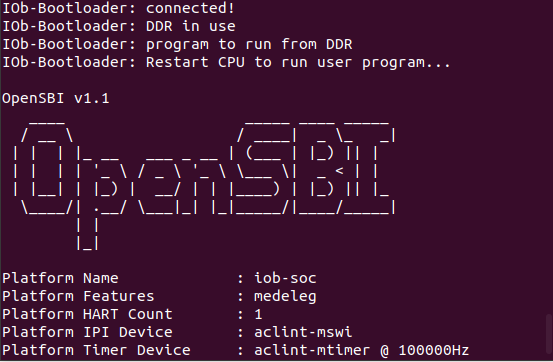
\includegraphics[width=0.5\textwidth]{../images/end_bootloader_sim.png}
    \caption{\textit{IOb-SoC} bootloader and \textit{OpenSBI} firmware.}
    \label{fig:end_bootloader_sim}
\end{figure}

Figure \ref{fig:start_bootloader_sim} shows the initialization of the \textit{Console} program. Furthermore, it shows the instantiation of the \textit{iob-UART16550} and the \textit{iob-PLIC}. The \textit{iob-UART16550} and the PLIC core have an initial block that prints their properties. The synthesis tools do not synthesise the initial block to real hardware, but the simulator executes it. Figure \ref{fig:end_bootloader_sim} shows the \textit{iob-bootloader} and the start of the \textit{OpenSBI} bootloader. The \textit{iob-bootloader} in figure \ref{fig:end_bootloader_sim} does not transfer the software to the memory because the author executed the simulation considering that the software was already in the memory.

Figure \ref{fig:start_linux_sim} shows the end of the \textit{OpenSBI} bootloader and the start of the Linux kernel. The first line printed by the Linux kernel indicates the author built the kernel executing, the kernel version and which toolchain he used to compile it.

\begin{figure}[!ht]
    \centering
    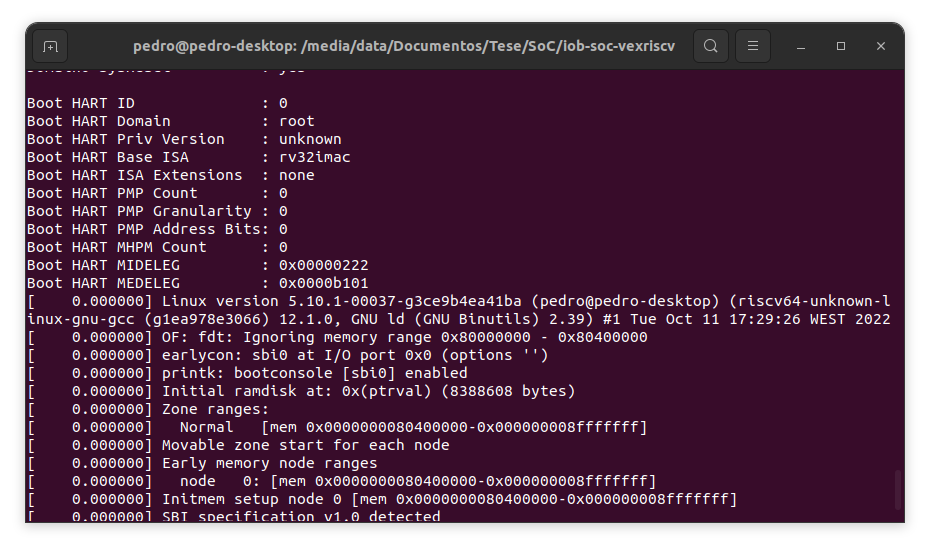
\includegraphics[width=0.5\textwidth]{../images/start_Linux_sim.png}
    \caption{Start of the Linux kernel boot with \textit{Verilator}.}
    \label{fig:start_linux_sim}
\end{figure}

While figure \ref{fig:start_linux_sim} shows the start of the Linux kernel, figure \ref{fig:end_linux_verilator} shows the end of the Linux kernel booting process and the execution of the "init" script. The "init" script is the first program the OS executes after the Linux kernel mounts the RootFS and finishes booting. There exist multiple messages printed to the terminal between the output shown in figure \ref{fig:start_linux_sim} and in \ref{fig:end_linux_verilator}. Those messages show the progress while the Linux kernel boots. The Linux kernel boot process's last message is "Run /init as init process". After that message the SoC executes the "init" program.

\begin{figure}[!ht]
    \centering
    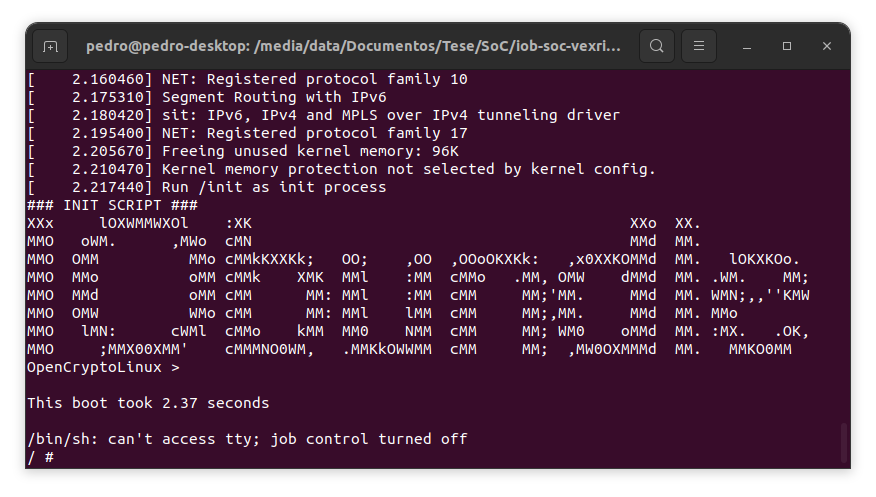
\includegraphics[width=0.5\textwidth]{../images/end_Linux_sim.png}
    \caption{End of Linux kernel boot with \textit{Verilator}.}
    \label{fig:end_linux_verilator}
\end{figure}

Figure \ref{fig:linux_fpga} shows the developed minimal OS running on an FPGA. The reader can see that the author has suppressed the shell warning. The initial part of the figure shows the final stage of the Linux kernel booting. After booting, the author tested the \textit{ls /} command that showed the files and directories in the systems' root. Lastly the author executed the \textit{cat init} command for the OS to print the contents of the "init" script to the terminal.

\begin{figure}[!ht]
    \centering
    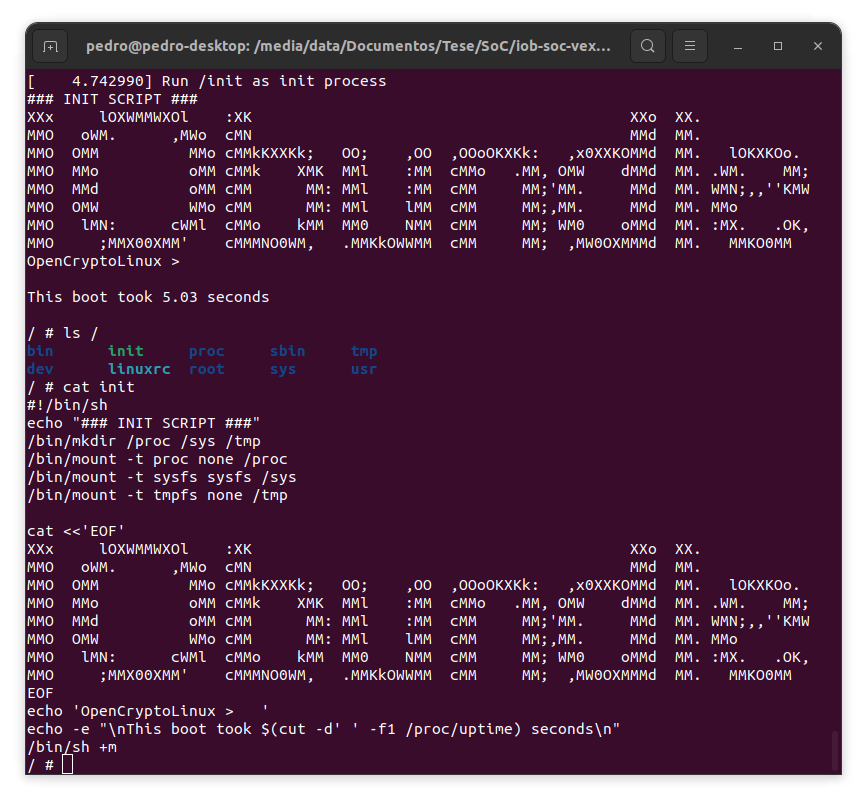
\includegraphics[width=0.5\textwidth]{../images/linux_fpga.png}
    \caption{Linux kernel boot in the FPGA.}
    \label{fig:linux_fpga}
\end{figure}

The time the Linux kernel takes to boot in real hardware, figure \ref{fig:linux_fpga}, is almost double what it takes to boot in simulation, figure \ref{fig:linux_fpga}. The time to boot is almost double because the memory module used in the simulation does not have any latency. When the L2 cache fetches data from memory in real hardware, it must wait before receiving the data burst. Using the \textit{CYCLONE V} FPGA board the Linux kernel takes 7.01 seconds to boot. The author expected the boot to take longer since the system clock frequency used with the \textit{CYCLONE V} is 50 MHz. The Kintex Ultrascale was able to run with a frequency of 100 MHz. The \textit{OpenSBI} bootloader and the device tree blob had to be recompiled with the system frequency defined to 50 MHz to run in the \textit{CYCLONE V}.

A more complex rootfs generated with \textit{Buildroot} provides more features than the minimal rootfs developed. The \textit{Buildroot} rootfs allows using \textit{MicroPython}~\cite{tollervey2017programming} in \textit{IOb-SoC-Linux} and executing the \textit{Dhrystones}~\cite{weicker1984dhrystone} benchmarking software. The rootfs size is a little over 2MB. Figure \ref{fig:linux_buildroot_fpga} shows the final output of the \textit{Dhrystones} benchmark and the execution of simple commands in \textit{MicroPython}. With the \textit{Buildroot} rootfs the Linux kernel takes 6.40 seconds to boot in the \textit{Kintex Ultrascale} and 8.14 seconds in the \textit{CYCLONE V}.

\begin{figure}[!ht]
    \centering
    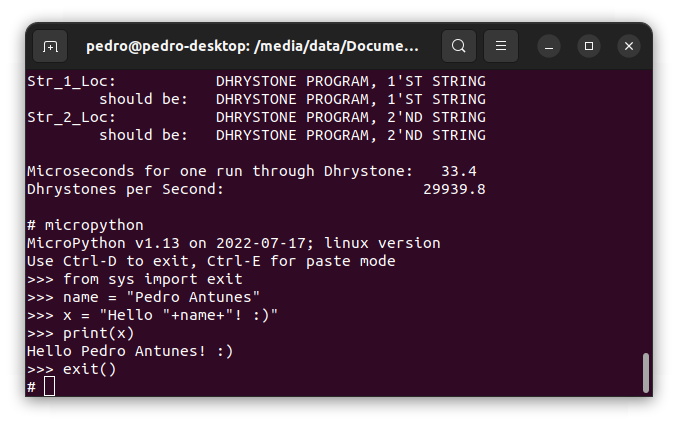
\includegraphics[width=\linewidth]{../images/linux_buildroot_fpga.png}
    \caption{Linux OS with \textit{Buildroot} rootfs.}
    \label{fig:linux_buildroot_fpga}
\end{figure}

\textit{MicroPython} is a software project that aims to implement a \textit{Python} version, highly compatible with \textit{Python3}, in microcontrollers and small embedded systems. \textit{Dhrystones} is a general-performance benchmarking software used in multiple embedded systems. With the \textit{Dhrystones} benchmark, developers can compare the efficiency of different computers or compilers. A common representation of the \textit{Dhrystones} benchmark is \textit{DMIPS}. \textit{DMIPS} is the number of \textit{Dhrystones} per Second divided by 1757, the number of \textit{Dhrystones} per second obtained on the \textit{VAX 11/780}~\cite{emer1984characterization}. Table \ref{tab:dhrystones} represents a comparison between the \textit{Dhrystones} benchmarking scores of both FPGA boards.

\begin{table}[!ht]
    \centering
    \begin{tabular}{l|l|l|}
    \cline{2-3}
                                                         & \textbf{Kintex Ultrascale} & \textbf{CYCLONE V} \\ \hline
    \multicolumn{1}{|l|}{One run through Dhrystone (ms)} & 24.4                       & 33.4               \\ \hline
    \multicolumn{1}{|l|}{Dhrystones per Second}          & 40983.2                    & 29939.8            \\ \hline
    \multicolumn{1}{|l|}{DMIPS}                          & 23.33                      & 17.04            \\ \hline
    \end{tabular}
    \caption{\textit{Dhrystones} benchmarking.}
    \label{tab:dhrystones}
\end{table}

Tables \ref{tab:kintex_linux} and \ref{tab:cyclone_linux} show the resources used by the \textit{IOb-SoC-Linux} in the different FPGAs.

\begin{table}[!ht]
    \centering
    \begin{tabular}{l|l|l|}
        \cline{2-3}
                                            & Resources & FPGA usage \% \\ \hline
        \multicolumn{1}{|l|}{ALM}         & 11,227    & 10                       \\ \hline
        \multicolumn{1}{|l|}{DSP}         & 8         & 3                        \\ \hline
        \multicolumn{1}{|l|}{FF}          & 13725     & 2                        \\ \hline
        \multicolumn{1}{|l|}{BRAM blocks} & 234       & 19                       \\ \hline
        \multicolumn{1}{|l|}{BRAM bits}   & 755,424   & 9                        \\ \hline
    \end{tabular}
    \caption{Cyclone V GT}
    \label{tab:cyclone_linux}
\end{table}
\begin{table}[!ht]
    \centering
    \begin{tabular}{l|l|l|}
        \cline{2-3}
                                        & Resources & FPGA usage \% \\ \hline
        \multicolumn{1}{|l|}{LUTs}      & 23126     & 9.54                     \\ \hline
        \multicolumn{1}{|l|}{Registers} & 24505     & 5.05                     \\ \hline
        \multicolumn{1}{|l|}{DSPs}      & 10        & 0.52                     \\ \hline
        \multicolumn{1}{|l|}{BRAM}      & 39.5      & 6.58                     \\ \hline
    \end{tabular}
    \caption{Kintex Ultrascale}
    \label{tab:kintex_linux}
\end{table}

Tables \ref{tab:kintex_linux} and \ref{tab:cyclone_linux} show that the resources utilization from the \textit{IOb-SoC-Linux} is not much bigger than the \textit{IOb-SoC}. The FPGA still has enough resources to implement hardware accelerators.
